%% bare_jrnl.tex
%% V1.4b
%% 2015/08/26
%%
%% Support sites:
%% http://www.michaelshell.org/tex/ieeetran/
%% http://www.ctan.org/pkg/ieeetran
%% and
%% http://www.ieee.org/



% *** Authors should verify (and, if needed, correct) their LaTeX system  ***
% *** with the testflow diagnostic prior to trusting their LaTeX platform ***
% *** with production work. The IEEE's font choices and paper sizes can   ***
% *** trigger bugs that do not appear when using other class files.       ***                          ***
% The testflow support page is at:
% http://www.michaelshell.org/tex/testflow/



\documentclass[journal]{IEEEtran}
%
%
\ifCLASSINFOpdf
  \usepackage[pdftex]{graphicx}
\else
  % DVI stuff 
\fi

% correct bad hyphenation here
\hyphenation{op-tical net-works semi-conduc-tor}


\begin{document}
%
\title{RISC-V: A Brief History}
%
\author{Saroj~Rout,~\IEEEmembership{Senior Member,~IEEE}\thanks{S. Rout is with Department of Electronics Engineering, Silicon Institute of Technology, Bhubaneswar, INDIA (see https://sroutk.github.io)} }% <-this % stops a space

% The paper headers
\markboth{Preprints in Technology Research at TechRxiv, November~2023}%
{Shell \MakeLowercase{\textit{et al.}}: RISC-V: A Brief History}

% make the title area
\maketitle

\begin{abstract}
This article briefly introduces the history behind the rise and popularity of the RISC-V instruction set architecture (ISA). It starts with a design of a microcontroller and how RISC-V fits into it. Then it briefly covers the history of microprocessor and emergence of RISC ISA and finally the opensource ISA, RISC-V.
\end{abstract}

% Note that keywords are not normally used for peerreview papers.
\begin{IEEEkeywords}
RISC-V, RISC, Computer Architecture
\end{IEEEkeywords}

%%%%%%%%%%%%%%%%%%%%%%%%%%%%%%%%%%%%%
% INTRODUCTION
%%%%%%%%%%%%%%%%%%%%%%%%%%%%%%%%%%%%%
\section{Introduction}

\IEEEPARstart{S}{ystems-on-a-chip} (SoC) with integrated processors are becoming ubiquitous. One such SoC is a microcontroller. It is hard to find a electronic system without a microcontroller in it eg. IoT, appliances, watches, toys and so on. They vary in complexity depending on the target applications. For example, Atmel's ATtiny series of microcontrollers are 8-bit processors starting with just 512-Bytes Flash and 32-Bytes of SRAM running at 10 MHz clock speed. On the other end of the spectrum are the STMicroelectronic's popular STM32 series microcontrollers which is based on Arm's Cortex-M 32-bit processor with up to 128 kB of L2 cache and and more than 600 kB of SRAM running at 650 MHz.

%%FIGURE : uC
\begin{figure}[htb]
    \centering
    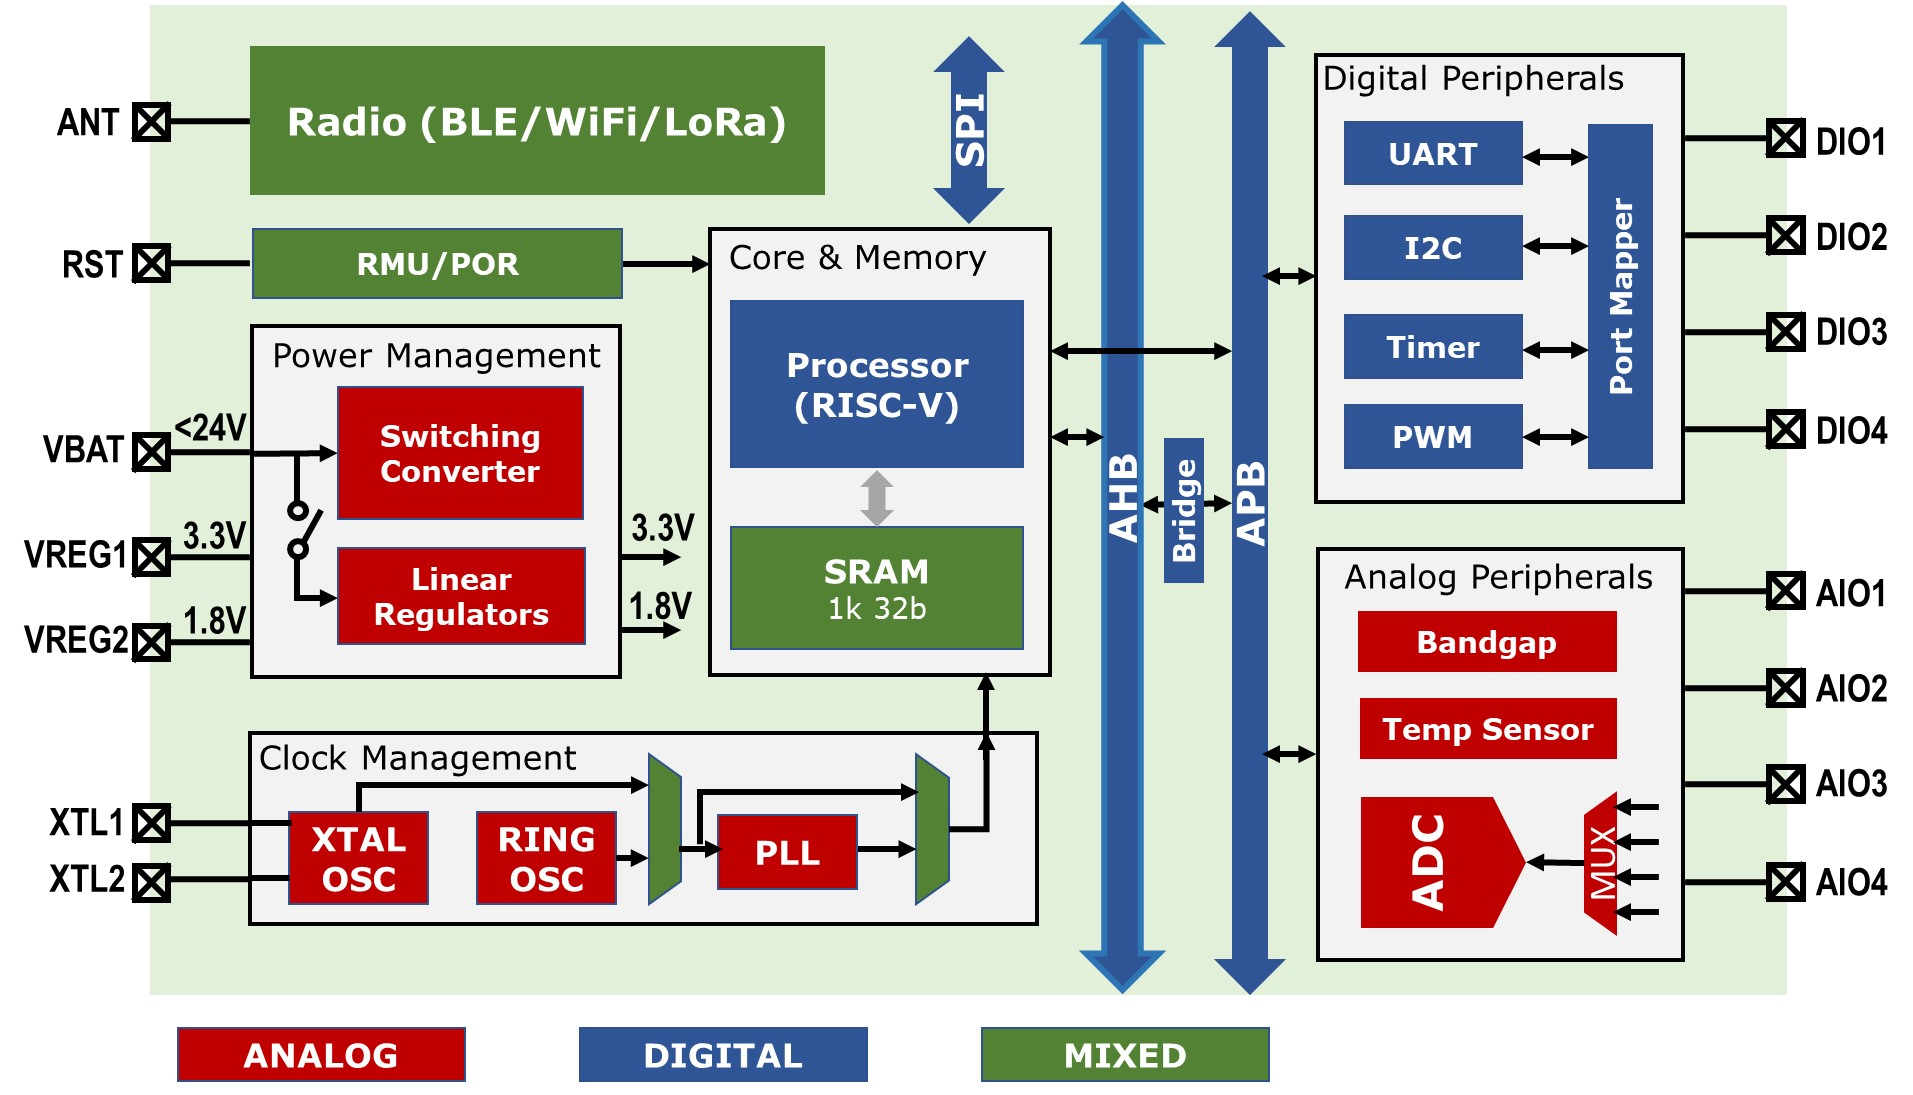
\includegraphics[width=0.95\linewidth]{image-uC.jpg}
    \caption{Architecture of a microcontroller intended for wireless IoT nodes.}
    \label{fig:uC}
\end{figure}

Fig.~\ref{fig:uC} shows an architecture of a microcontroller intended for IoT wireless nodes. It contains a core processor, a cache (SRAM), analog peripherals (bandgap voltage reference, temperature sensor and analog-to-digital converter(ADC) ), digital peripherals (UART, SPI, PWM), power management, clock management (PLL, crystal oscillator), and RF Radio (Bluetooth, WiFi, LoRa). Apart from the processor, all other blocks (typically called IPs) can either be designed from scratch by mixed-signal engineers or licensed from a vendor. When it comes to the processor, it gets a little complicated. You can use a very old instruction set architecture (ISA) and implement it in your target technology. One such popular ISA is Intel's 8051 microcontroller architecture developed in 1980s. It has been around for several decades and has proven to be reliable, efficient, and versatile. Its compact size, low power consumption, and wide range of peripherals make it a popular choice for many embedded systems applications. Additionally, there is a large community of developers and engineers who are familiar with the 8051 architecture, which makes it easier to find support and resources for development.

Companies like Arm, IBM and Intel have very successful ISAs but patents on key aspects of their ISAs prevent others from using them without licenses which imposes a prohibitive cost for most educational, research organization or companies trying to target low-volume markets. 
Note, ISA is neither an implementation of the hardware or the software (OS, drivers, compilers). It is a standardization of the interface specification so development tools and design implementations can be reused and shared provided they are open and free. And, both hardware and software can be implemented in three ways: proprietary, licensed open-source, or free open-source.

There are three free and open-source RISC ISAs currently available for use:
\begin{enumerate}
    \item \emph{SPARC V8} from Sun Microsystems that was made into a IEEE standard in 1994.
    \item \emph{OpenRISC} is a GNU open-source effort started in 2000, with the 64-bit ISA being completed in 2011.
    \item \emph{RISC-V} (pronounced "RISC 5") a BSD open-source effort started in 2010 at University of California at Berkeley by Krste Asanović, David A. Patterson and their graduate students Andrew Waterman and Yunsup Lee  partly inspired by ARM's IP restrictions together with the lack of 64-bit addresses and overall baroqueness of ARM v7.
\end{enumerate}

Before we look at the history of RISC-V and why it prospered compared to it's predecessors SPARC V8 and OpenRISC, it's worth taking a quick look at the history of microprocessors and how RISC has emerged as the goto architecture for power-conscious devices such as tablets, mobile phones and embedded systems.

%%%%%%%%%%%%%%%%%%%%%%%%%%%%%%%%%%%%%
% BRIEF HISTORY OF MICROPROCESSORS
%%%%%%%%%%%%%%%%%%%%%%%%%%%%%%%%%%%%%
\section{Brief History of Microprocessors}

The birth of microprocessor took around the end of 1960s when a Japanese calculator maker Business Computer Corporation (Busicom) contracted with Intel, then a small startup, for custom chips for a calculator. That gave birth to Intel 4004 which is widely accepted as the first microprocessor and that calculator was launched in early 1971 with the Intel 4004 in it along with chips for storage and I/O. In early 1970, Computer Terminal Corporation (CTC), a company based in San Antonio, TX, USA, arranged Intel to build a single MOS chip to replace their discrete-based 8-bit processor for their general purpose computer, Data Point 2200. Although Intel went ahead and build the chip based on the Data Point 2200 architecture, the project got suspended as CTC contracted Texas Instruments (TI) for the job \footnote{An interesting historical note: Intel was a startup with about 100 employees and Texas Instruments was a large company with more than 45,000 employees.}. TI developed the TMC 1795 processor for CTC which was rejected after testing the chip. Eventually TI abandoned the project after failing to market it to other companies. In the mean time, Intel 8008 was successfully working at the end of 1971, but CTC had lost interest in that project an gave up its exclusive right to design. Intel then commercialized 8008 in April 1972, and went on to become a successful product. In 1974 the 8008 spawned the Intel 8080, which in turn heavily influenced the Intel 8086 and today's x86 architecture which went on to dominate the personal computer (PC) and the server market. So the history is certainly very interesting where it all started with CTC's Data Point 2200 computer which eventually established Intel as a microprocessor company and its x86 architecture as a leading architecture in the years ahead.

From 1978 till 1988, Complex Instruction Set Computer (CISC) architecture dominated the market with the performance improvement averaging at 15\% per year. This improvement mainly owed to the Moore's Law which ensured the doubling of transistors per unit area every 18 months and Dennard's scaling theory to ensure that power consumed in the chip also reamained about the same.

From 1988-2003, focus shifted to improving single-processor performance by exploiting instruction level parallelism (ILP) which led to Reduced Instruction Set Computer (RISC) architecture becoming mainstream. Single processor performance improved tremendously with the use of pipelining for single-cylce execution, branch prediction, out-of-order execution, on-chip caches, multi-level on-chip caches, superscalar processors, VLIW. Continuing benefit of Moore’s law and Dennard scaling performance improvement averaged @ 40 \% per year.
This perfomance enhancement was result of RISC Instruction Set Architecture (ISA) change and microarchitectures based on pipelined execution. RISC offered a simplified ISA that restricted arithmetic and logic operations to register operands as source and destination operands. Memory access was limited to two instructions, load and store, without performing any logic or arithmetic operation on the operands. The memory addressing modes were fewer and simpler compared to CISC. The RISC ISA also allowed for ILP through pipelining of instructions that gives a throughput of one instruction per cycle in contrast with a CISC architecture taking multiple cycle for an instruction to execute. Additionally, RISC ISA also allowed for Superscalar Processing where more than one isntruction can be fed to the pipeline in parallel albeit some challenges involved in doing so.

 

% Can use something like this to put references on a page
% by themselves when using endfloat and the captionsoff option.
\ifCLASSOPTIONcaptionsoff
  \newpage
\fi


\begin{thebibliography}{1}

\bibitem{IEEEhowto:kopka}
H.~Kopka and P.~W. Daly, \emph{A Guide to \LaTeX}, 3rd~ed.\hskip 1em plus
  0.5em minus 0.4em\relax Harlow, England: Addison-Wesley, 1999.

\end{thebibliography}

% that's all folks
\end{document}


%%*************************************************************************
%% Legal Notice:
%% This code is offered as-is without any warranty either expressed or
%% implied; without even the implied warranty of MERCHANTABILITY or
%% FITNESS FOR A PARTICULAR PURPOSE! 
%% User assumes all risk.
%% In no event shall the IEEE or any contributor to this code be liable for
%% any damages or losses, including, but not limited to, incidental,
%% consequential, or any other damages, resulting from the use or misuse
%% of any information contained here.
%%
%% All comments are the opinions of their respective authors and are not
%% necessarily endorsed by the IEEE.
%%
%% This work is distributed under the LaTeX Project Public License (LPPL)
%% ( http://www.latex-project.org/ ) version 1.3, and may be freely used,
%% distributed and modified. A copy of the LPPL, version 1.3, is included
%% in the base LaTeX documentation of all distributions of LaTeX released
%% 2003/12/01 or later.
%% Retain all contribution notices and credits.
%% ** Modified files should be clearly indicated as such, including  **
%% ** renaming them and changing author support contact information. **
%%*************************************************************************
